\documentclass[tikz,border=4pt]{standalone}
\usepackage[T1]{fontenc}
\usepackage[scaled=0.92]{helvet}
\usepackage{amsmath,amssymb}
\usepackage{tikz}
\usetikzlibrary{arrows.meta,positioning,shapes.geometric,shapes.misc,calc,fit,backgrounds}

\begin{document}
\sffamily
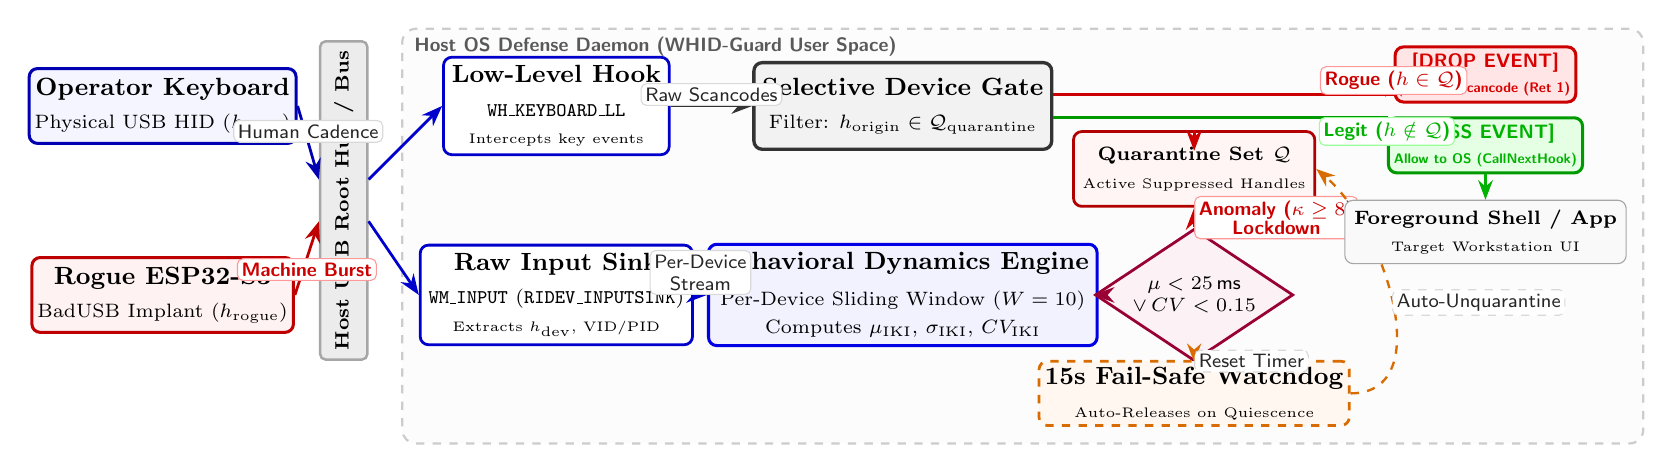
\begin{tikzpicture}[
    >=Stealth,
    font=\small,
    % Device blocks
    dev_rogue/.style={
        rectangle,
        rounded corners=3pt,
        draw=red!75!black,
        line width=1.1pt,
        fill=red!5!white,
        minimum width=2.5cm,
        minimum height=0.95cm,
        inner sep=2pt,
        align=center
    },
    dev_legit/.style={
        rectangle,
        rounded corners=3pt,
        draw=blue!70!black,
        line width=1.1pt,
        fill=blue!4!white,
        minimum width=2.5cm,
        minimum height=0.95cm,
        inner sep=2pt,
        align=center
    },
    % Module block
    mod_block/.style={
        rectangle,
        rounded corners=3pt,
        draw=blue!80!black,
        line width=1.0pt,
        fill=white,
        minimum width=2.3cm,
        minimum height=1.0cm,
        inner sep=3pt,
        align=center
    },
    % Engine block
    eng_block/.style={
        rectangle,
        rounded corners=3pt,
        draw=blue!90!black,
        line width=1.1pt,
        fill=blue!5!white,
        minimum width=2.7cm,
        minimum height=1.2cm,
        inner sep=3pt,
        align=center
    },
    % Decision Diamond
    decision/.style={
        diamond,
        aspect=1.5,
        draw=purple!80!black,
        line width=1.0pt,
        fill=purple!5!white,
        inner sep=1.5pt,
        align=center,
        font=\sffamily\scriptsize
    },
    % Gate switch
    gate_block/.style={
        rectangle,
        rounded corners=3pt,
        draw=black!80,
        line width=1.2pt,
        fill=gray!10!white,
        minimum width=2.3cm,
        minimum height=1.1cm,
        inner sep=3pt,
        align=center
    },
    % Action pills
    pill_drop/.style={
        rectangle,
        rounded corners=3pt,
        draw=red!80!black,
        line width=1.1pt,
        fill=red!10!white,
        minimum width=2.2cm,
        minimum height=0.7cm,
        inner sep=2pt,
        align=center,
        font=\sffamily\scriptsize\bfseries,
        text=red!85!black
    },
    pill_pass/.style={
        rectangle,
        rounded corners=3pt,
        draw=green!60!black,
        line width=1.1pt,
        fill=green!10!white,
        minimum width=2.2cm,
        minimum height=0.7cm,
        inner sep=2pt,
        align=center,
        font=\sffamily\scriptsize\bfseries,
        text=green!70!black
    },
    % Watchdog
    wdt_block/.style={
        rectangle,
        rounded corners=3pt,
        draw=orange!85!black,
        line width=1.0pt,
        dashed,
        fill=orange!6!white,
        minimum width=2.4cm,
        minimum height=0.8cm,
        inner sep=2pt,
        align=center
    },
    % Badges
    lbl/.style={
        font=\sffamily\scriptsize,
        fill=white,
        draw=gray!30,
        line width=0.4pt,
        rounded corners=2pt,
        inner sep=1.5pt,
        align=center,
        text=black!85
    },
    lbl_red/.style={
        font=\sffamily\scriptsize\bfseries,
        fill=white,
        draw=red!40,
        line width=0.4pt,
        rounded corners=2pt,
        inner sep=1.5pt,
        align=center,
        text=red!80!black
    },
    lbl_green/.style={
        font=\sffamily\scriptsize\bfseries,
        fill=white,
        draw=green!40,
        line width=0.4pt,
        rounded corners=2pt,
        inner sep=1.5pt,
        align=center,
        text=green!70!black
    }
]

% ==============================================================================
% Column 1: Physical Peripherals (x = 0)
% ==============================================================================
\node[dev_legit] (kb_legit) at (0, 1.2) {\textbf{Operator Keyboard}\\[1pt]\scriptsize Physical USB HID ($h_{\text{legit}}$)};
\node[dev_rogue] (badusb)   at (0, -1.2) {\textbf{Rogue ESP32-S3}\\[1pt]\scriptsize BadUSB Implant ($h_{\text{rogue}}$)};

% USB Bus Node (x = 2.4)
\node[rectangle, draw=gray!70, fill=gray!15, line width=0.9pt, minimum width=0.6cm, minimum height=3.2cm, rounded corners=2pt, align=center] (bus) at (2.3, 0) {\rotatebox{90}{\scriptsize\textbf{Host USB Root Hub / Bus}}};

\draw[->, line width=1.0pt, draw=blue!70!black] (kb_legit.east) -- node[above, lbl] {Human Cadence} (bus.140);
\draw[->, line width=1.0pt, draw=red!75!black]  (badusb.east)   -- node[below, lbl_red] {Machine Burst} (bus.220);

% ==============================================================================
% Column 2: Ingestion Dual Channels (x = 4.8)
% ==============================================================================
% Channel A: Low-Level Hook Interception (Top)
\node[mod_block] (hook) at (5.0, 1.2) {\textbf{Low-Level Hook}\\[1pt]\scriptsize \texttt{WH\_KEYBOARD\_LL}\\[-1pt]\tiny Intercepts key events};

% Channel B: Raw Input Telemetry (Bottom)
\node[mod_block] (rawinput) at (5.0, -1.2) {\textbf{Raw Input Sink}\\[1pt]\scriptsize \texttt{WM\_INPUT} (\texttt{RIDEV\_INPUTSINK})\\[-1pt]\tiny Extracts $h_{\text{dev}}$, VID/PID};

\draw[->, line width=1.0pt, draw=blue!80!black] (bus.40) -- (hook.west);
\draw[->, line width=1.0pt, draw=blue!80!black] (bus.320) -- (rawinput.west);

% ==============================================================================
% Column 3: Telemetry Processing & Anomaly Engine (x = 9.2)
% ==============================================================================
\node[eng_block] (engine) at (9.4, -1.2) {\textbf{Behavioral Dynamics Engine}\\[2pt]\scriptsize Per-Device Sliding Window ($W=10$)\\[-1pt]\scriptsize Computes $\mu_{\text{IKI}}$, $\sigma_{\text{IKI}}$, $CV_{\text{IKI}}$};

\draw[->, line width=1.0pt, draw=blue!80!black] (rawinput.east) -- node[above, lbl] {Per-Device\\Stream} (engine.west);

% Decision Diamond (x = 13.0, y = -1.2)
\node[decision] (decision_box) at (13.1, -1.2) {$\mu < 25\,\text{ms}$\\$\lor\,CV < 0.15$};

\draw[->, line width=1.0pt, draw=purple!80!black] (engine.east) -- (decision_box.west);

% ==============================================================================
% Column 4: Selective Quarantine Gate & Watchdog (Top & Right)
% ==============================================================================
% Selective Gate (x = 9.4, y = 1.2)
\node[gate_block] (gate) at (9.4, 1.2) {\textbf{Selective Device Gate}\\[1pt]\scriptsize Filter: $h_{\text{origin}} \in \mathcal{Q}_{\text{quarantine}}$};

\draw[->, line width=1.0pt, draw=black!80] (hook.east) -- node[above, lbl] {Raw Scancodes} (gate.west);

% Quarantine State Table (x = 13.1, y = 1.2)
\node[rectangle, rounded corners=3pt, draw=red!70!black, line width=1.0pt, fill=red!4!white, minimum width=2.2cm, minimum height=0.95cm, align=center] (qset) at (13.1, 0.4) {\scriptsize\textbf{Quarantine Set $\mathcal{Q}$}\\[-1pt]\tiny Active Suppressed Handles};

% Feedback from Decision to Quarantine Set
\draw[->, line width=1.1pt, draw=red!80!black] (decision_box.north) -- node[right, lbl_red] {Anomaly ($\kappa \ge 8$)\\[-1pt]Lockdown} (qset.south);
\draw[->, line width=1.0pt, draw=red!80!black] (qset.north) -- (gate.south -| qset.north);

% Watchdog fail-safe timer (x = 13.1, y = -2.5)
\node[wdt_block] (wdt) at (13.1, -2.45) {\textbf{15s Fail-Safe Watchdog}\\[1pt]\tiny Auto-Releases on Quiescence};
\draw[->, line width=0.85pt, dashed, draw=orange!85!black] (wdt.north) -- node[right, lbl] {Reset Timer} (decision_box.south);
\draw[->, line width=0.85pt, dashed, draw=orange!85!black] (wdt.east) to[out=0, in=-40] node[right, lbl] {Auto-Unquarantine} (qset.east);

% ==============================================================================
% Column 5: Dual Enforcement Outputs (x = 16.6)
% ==============================================================================
\node[pill_drop] (drop_out) at (16.8, 1.6) {\textbf{[DROP EVENT]}\\[1pt]\tiny Suppress scancode (Ret 1)};
\node[pill_pass] (pass_out) at (16.8, 0.7) {\textbf{[PASS EVENT]}\\[1pt]\tiny Allow to OS (CallNextHook)};

\draw[->, line width=1.1pt, draw=red!80!black] ([yshift=4pt]gate.east) -| node[above, lbl_red] {Rogue ($h \in \mathcal{Q}$)} (drop_out.west);
\draw[->, line width=1.1pt, draw=green!60!black] ([yshift=-4pt]gate.east) -| node[below, lbl_green] {Legit ($h \notin \mathcal{Q}$)} (pass_out.west);

% Target OS Application Focus Box
\node[rectangle, rounded corners=3pt, draw=gray!70, fill=gray!5, minimum width=2.4cm, minimum height=0.7cm, align=center] (target_app) at (16.8, -0.4) {\scriptsize\textbf{Foreground Shell / App}\\[-1pt]\tiny Target Workstation UI};

\draw[->, line width=0.9pt, draw=green!70!black] (pass_out.south) -- (target_app.north);

% Background Container: Host OS User Space
\begin{scope}[on background layer]
    \node[rectangle, draw=gray!40, dashed, fill=gray!2, line width=0.8pt, rounded corners=5pt,
          fit=(hook) (rawinput) (engine) (decision_box) (gate) (qset) (wdt) (drop_out) (pass_out) (target_app),
          inner sep=6pt] (host_bg) {};
    \node[anchor=north west, font=\sffamily\bfseries\scriptsize, text=gray!70!black] at (host_bg.north west) {\,Host OS Defense Daemon (WHID-Guard User Space)};
\end{scope}

\end{tikzpicture}
\end{document}
